\documentclass{article}
\usepackage{tikz}
% These libraries give us shapes, modern arrows, and relative positioning
\usetikzlibrary{shapes.geometric, arrows.meta, positioning}

\begin{document}

% 1. Define the styles for your boxes so you don't repeat yourself
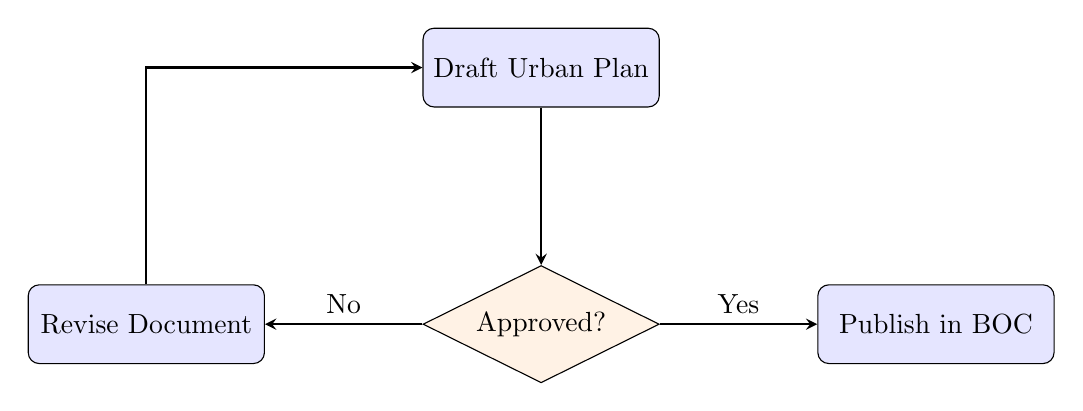
\begin{tikzpicture}[
    node distance=2cm and 2cm, % Vertical and Horizontal spacing
    process/.style={rectangle, rounded corners, minimum width=3cm, minimum height=1cm, text centered, draw=black, fill=blue!10},
    decision/.style={diamond, aspect=2, minimum width=3cm, minimum height=1cm, text centered, draw=black, fill=orange!10},
    arrow/.style={thick, ->, >=stealth} % Modern stealth arrows
]

% 2. Place the Nodes (the boxes)
\node (start)   [process] {Draft Urban Plan};
\node (review)  [decision, below=of start] {Approved?};
\node (publish) [process, right=of review] {Publish in BOC};
\node (revise)  [process, left=of review] {Revise Document};

% 3. Draw the Arrows
\draw [arrow] (start) -- (review);
\draw [arrow] (review) -- node[anchor=south] {Yes} (publish);
\draw [arrow] (review) -- node[anchor=south] {No} (revise);
\draw [arrow] (revise) |- (start); % The |- draws a right-angle line!

\end{tikzpicture}

\end{document}